\documentclass[]{scrartcl}

%opening
\title{Theoretical Background for Globe Thermometers}
\author{Finn Huybrechts \& Noah Verhoeven}

\usepackage[dutch]{babel}
\usepackage{amsmath,amssymb,amsfonts,textcomp}
\usepackage{caption}
\usepackage{listings}
\usepackage{subcaption}
\usepackage{wrapfig}
\usepackage{yhmath}
\usepackage{textcomp}
\usepackage{booktabs}
\usepackage{graphicx}
\usepackage{float,flafter}
\usepackage[colorlinks=true]{hyperref}
\usepackage{inputenc}
\usepackage{multirow}
\usepackage{biblatex}
\usepackage{pxfonts}
\usepackage{mathtools}
\usepackage{diffcoeff}
\usepackage{siunitx}
\usepackage{physics}
\usepackage{wasysym}
\usepackage{sectsty}


\begin{document}
\maketitle

This documents serves as a theoretical background for the working of a globe thermometer, and how it relates to the mean radiant temperature. The results here have been independently found, with help from our course in thermal physics and the book "Introduction to Heat Transfer" by B. Sundén.

\section{Black Globe Thermometers}
The Mean Radiant Temperature (MRT) $T_{\text{MRT}}$ is defined as the temperature a fictive perfect black body would need such that the net energy exchange with a subject inside is the same as the environment. If a human, due to the thermal radiation of the environment, absorbs the $S_{\text{env}}$ radiation flux density, than $T_{\text{MRT}}$ is the temperature our fictive black body would need to equal this absorbed energy. Assuming the human body is a grey body, meaning the absorption coefficient is constant, we emphasize the following relationship
\begin{equation}\label{eq:emphasis}
	S_{\text{env}} = a_{h}\sigma T^4_{\text{MRT}}
\end{equation}
Where $a_{h}$ is the absorption coefficient of the human body, in general, this coefficient is wavelength dependent, which we'll come back to later. We also note that $\left[S_{\text{env}}\right] = \unit{\watt\per\meter\squared} = \unit{\joule\per\second\per\meter\squared}$.


\subsection{Radiative Heat Exchange}
We now derive a formula to determine $T_{\text{MRT}}$ with a globe thermometer. First, imagine a black ($\epsilon\approx1$) globe thermometer, such that all incident radiation is absorbed, without considering other heat exchanges. If the human body absorbs $S_{\text{env}}$ radiation, than the incident radiation flux density from the environment $E_{\text{env}}$ must be $\frac{S_{\text{env}}}{a_{h}}$. This thermal radiation will all be absorbed by our black globe thermometer. As it heats up, it will start emitting more (energetic) thermal radiation. The change in the energy over time of our globe thermometer is
\begin{equation}\label{eq:ideal}
	\boxed{\dot{Q} = A\left(\frac{S_{\text{env}}}{a_{h}} - \sigma T^4_g\right) = A\left(\sigma T^4_{\text{MRT}} - \sigma T^4_g\right)}
\end{equation}
With $A$ the surface of our globe thermometer, we emphasize that $\left[\dot{Q}\right] = \unit{\joule\per\second}$. We substituted equation \eqref{eq:emphasis} and used Stefan-Boltzmann's law to obtain the energy the globe thermometer would lose (emit) due to thermal radiation. Note that $\dot{Q}$ is $\lambda$-independent, which is because this theoretical exchange is between perfect black/grey bodies. \textbf{We can conceptually view this as the globe thermometer being stuck inside our fictive black body}. Eventually, an equilibrium is reached such that our globe thermometer has a stable temperature, at this point the globe thermometer emits as much thermal radiation as it receives, and thus it follows that $\dot{Q}=0$. We conclude from this that, at equilibrium, the globe temperature $T_g$ in these idealized conditions relates to $T_{\text{MRT}}$ as
\begin{equation}\label{eq:zeroth-condition}
	\text{Equilibrium (only radiative exchange):}\quad T_\text{MRT} = T_g
\end{equation}
In these idealized conditions we could, therefore, wait until the globe thermometer has reached equilibrium and measure its temperature to obtain $T_{\text{MRT}}$.
\\
\subsection{Convective Heat Exchange}
However, in the real world our globe thermometer will also exchange heat due to convection. We'll start by first imaging our globe thermometer in non-moving air with a temperature $T_a$. For this, we first note that if the air temperature $T_a$ is above that of our globe thermometer ($T_a > T_{g}$), than the globe thermometer will keep heating up. Because of this, the thermal radiation it emits will be greater than that of our fictive perfect black body. We thus note that
\begin{equation}\label{eq:first-condition}
	\text{Equilibrium ($T_a > T_g$):}\quad T_\text{MRT} < T_g
\end{equation}
Analogously, if the air temperature is lower than that of the globe thermometer ($T_a < T_g$), than the globe thermometer will cool down and reach an equilibrium at a temperature below $T_{\text{MRT}}$, and thus
\begin{equation}\label{eq:second-condition}
	\text{Equilibrium ($T_a < T_g$):}\quad T_\text{MRT} > T_g
\end{equation}
The combination of \eqref{eq:zeroth-condition}, \eqref{eq:first-condition} and \eqref{eq:second-condition} provide physically intuitive 'constraints', which can be used to check if our solution makes physical sense.
\\

We now employ thermodynamics to find the flow of heat due to convection, it is a standard result that
\begin{equation}
	\dot{Q}_\text{con} = hA\Delta T = hA\left(T_g - T_a\right)
\end{equation}
We can add this additional heat exchange term to \eqref{eq:ideal}. Assuming equilibrium again, we set $\dot{Q} = 0$, resulting in
\begin{equation}\label{eq:final-black}
	\boxed{A\sigma T^4_{\text{MRT}} = A\sigma T^4_g + hA\left(T_g - T_a\right) \quad \Longrightarrow \quad T_{\text{MRT}} = \left[T_g^4 + \frac{h}{\sigma}\left(T_g - T_a\right)\right]^{\frac{1}{4}}}
\end{equation}
With $h$ the convective heat transfer coefficient. We check if this solution makes physical sense. Indeed, constraints \eqref{eq:zeroth-condition}, \eqref{eq:first-condition} and \eqref{eq:second-condition} are all fulfilled in their respective scenarios. Now, the difficulty lies in determining $h$, as this coefficient usually depends on temperature and the type of convection (free vs forced, laminar vs turbulence).

\section{Grey Globe Thermometers}
Equation \eqref{eq:final-black} effectively provides the necessary parameters to measure when using a black globe thermometer. We found that both globe thermometer $T_g$ and air $T_a$ temperatures need to be actively monitored. Additionally, depending on the type of convection, and the setting where this takes place, the convective heat transfer coefficient should be derived (and the necessary quantities monitored).
\\

However, in the real world our globe won't be perfectly black, and will, for example, always have some reflectivity. Therefore, instead of assuming a perfectly black globe thermometer, we now assume a perfectly grey globe, meaning the absorptivity $a_{g}$ and emmisivity $\epsilon_g$ are constant.

\subsection{Radiative Heat Exchange}
We, again, start from the idealized setting were only radiative heat exchange is possible. Because our globe is now grey, it won't perfectly emit or absorb. We account for this by introducing the aforementioned absorptivity and emmisivity in \eqref{eq:ideal}, we find
\begin{equation}\label{eq:ideal-grey}
	\boxed{\dot{Q} = A\left(a_g\frac{S_{\text{env}}}{a_{h}} - \epsilon_g\sigma T^4_g\right) = A\left(a_g\sigma T^4_{\text{MRT}} - \epsilon_g\sigma T^4_g\right)}
\end{equation}
According to Kirchhoff's law\footnote{We don't just substitute these values to put emphasize on which quantities are responsible for emission and absorption.}, it holds that $\epsilon_{g} = a_{g}$. Using this we easily find that the same equilibrium \eqref{eq:zeroth-condition} holds for both grey- and black globe thermometers.

\subsection{Convective Heat Exchange}
Employing similar reasoning, we easily find that both \eqref{eq:first-condition} and \eqref{eq:second-condition} also hold in the grey globe thermometer case. Our final expression now becomes
\begin{equation}
	\boxed{Aa_g\sigma T^4_{\text{MRT}} = A\epsilon_g\sigma T^4_g + hA\left(T_g - T_a\right) \quad \Longrightarrow \quad T_{\text{MRT}} = \left[T_g^4 + \frac{h}{a_g\sigma}\left(T_g - T_a\right)\right]^{\frac{1}{4}}}
\end{equation}
Which is in agreement with relevant literature. A recommended formula for $h$ is given by McAdams (1954).



\section{Spectral Emmisivity}
\subsection{Definition}
In the previous sections we assumed perfect black/grey globe thermometers, meaning the absorptivity and emmisivity were constant. However, in reality, the absorptivity is a function of wavelength $\lambda$. We first introduce the definition of emmisivity, which is the fraction between the radiation flux density $E$ of the real object and the radiation flux a perfect black body $E_B$ of the same temperature would produce
$$
\epsilon(\lambda, T) = \frac{E(\lambda, T)}{E_B(\lambda, T)}
$$
From this we find that the wavelength $\lambda$ and temperature $T$ dependent radiation flux of the real object is given by
$$
E(\lambda, T) = \epsilon(\lambda, T)E_B(\lambda, T)
$$
We obtain the total radiation flux by integrating over all wavelengths
\begin{equation}\label{eq:definition}
	E(T) = \int_{0}^\infty\epsilon(\lambda, T) E_B(\lambda, T) d\lambda
\end{equation}
We check if this definition matches our previously used results, indeed, if $\epsilon(\lambda, T)$ is constant (regarding $\lambda$), we find
$$
E(T) = \epsilon(T)\int_{0}^\infty E_B(\lambda, T) d\lambda = \epsilon(T)\sigma T^4
$$
Where this integral is the known result for a perfect black body. In the following, we will assume the temperature to be of negligible impact, which is physically justified in the temperature ranges we are considering. This simplifying assumption is also supported by the literature. 

\subsection{New Equilibrium Condition}
Because the emmisivity and absorptivity are now $\lambda$-dependent quantities, it follows that with each wavelength $\lambda$ a 'separate' heat exchange can be associated. Therefore, we now require, to reach equilibrium, that the total heat exchange over time stays consistent, or
\begin{equation}\label{eq:new-condition}
	\text{Equilibrium condition:} \quad \boxed{\dot{Q} = \int_{0}^{\infty}\dot{Q}_\lambda(\lambda) d\lambda = 0}
\end{equation}
With $\dot{Q}_\lambda$ the specific heat exchange in the interval $\left[\lambda, \lambda + d\lambda \right]$.
\\

This condition should reduce to our previous condition as our globe thermometer becomes perfectly black/grey. Indeed, for a perfectly black/grey globe $\dot{Q}$ will be $\lambda$-independent, as we noted earlier. We therefore find the equilibrium condition
$$
\dot{Q} = \dot{Q}_\lambda \int_{0}^{\infty}d\lambda = 0$$
Which can only be satisfied when $\dot{Q}=\dot{Q}_\lambda = 0$.

\subsection{Radiative Heat Exchange}
We, again, start by only considering radiative heat exchange. The radiation emitted by our globe thermometer $E_g$ can be written, according to \eqref{eq:definition}, as
$$
E_g(T_g) = \int_{0}^\infty\epsilon_g(\lambda) E_B(\lambda, T_g) d\lambda
$$
With $T_g$ the globe temperature and $\epsilon_g(\lambda)$ the globe emmisivity. Now imagine that the environment produces a radiation flux density $E_{\text{env}}(\lambda)$, than the amount of this radiation the human body absorbs $S_{\text{env}}$ necessarily abids by
\begin{equation}\label{necessary}
	\boxed{S_{\text{env}} = \int_{0}^\infty a_h(\lambda)E_{\text{env}}(\lambda) d\lambda = \int_{0}^{\infty} a_h(\lambda) E_B(\lambda, T_{\text{MRT}})d\lambda}
\end{equation}
With $a_h(\lambda)$ absorptivity of the human body. This last term appears by definition, since we want our fictive black body to have a temperature $T_{\text{MRT}}$ such that it matches $S_{\text{env}}$. From this expression we can derive our previously used results. If we again assume $a_h$ to be constant ($a_h(\lambda) = a_h$), than we find that $$
\frac{S_{\text{env}}}{a_h}=\int_{0}^\infty E_{\text{env}}(\lambda) d\lambda =\int_{0}^{\infty} E_B(\lambda, T_{\text{MRT}})d\lambda = \sigma T^4_{\text{MRT}}
$$
Which is exactly what we used.
\\

We now put our globe thermometer in this same environment, as such the incident radiation is $E_{\text{env}}(\lambda)$, from which $I_g$ will be absorbed by our globe, we express this as
\begin{equation}\label{incident}
	I_g = \int_{0}^{\infty} a_g(\lambda) E_{\text{env}}(\lambda) d\lambda
\end{equation}
With $a_g(\lambda)$ the globe absorptivity. Considering our new equilibrium condition \eqref{eq:new-condition}, and putting together the emission and absorption, we find that at equilibrium
$$
\dot{Q} = A\left(I_g - E_g\right) = 0 \quad \Longrightarrow \quad \int_{0}^{\infty} a_g(\lambda) E_{\text{env}}(\lambda) d\lambda = \int_{0}^\infty\epsilon_g(\lambda) E_B(\lambda, T_g) d\lambda
$$
Using Kirchhoff's law ($a(\lambda) = \epsilon(\lambda)$) we can write that, in the general case, equilibrium in our globe thermometer is reach when
\begin{equation}\label{general}
	\boxed{\int_{0}^{\infty}\epsilon_g(\lambda)\left(E_{\text{env}}(\lambda) - E_B(\lambda, T_g)\right)d\lambda = 0}
\end{equation}
Which is a somewhat initiative result.  
\\

\subsubsection{Special Case: Matching Spectral Emmisivity}
In order to obtain $T_{\text{MRT}}$ from \eqref{general}, we need to employ equation \eqref{necessary}. As we'll see shortly, an analytical way of eliminating $E_{\text{env}}$ from this identity is impossible. If, however, we assume the special case were the spectral emmisivity (and absorptivity) of our globe matches that of the human body, or
$$
\text{Special case:} \quad a_h(\lambda) = a_g(\lambda) \quad \Longrightarrow\quad a_h(\lambda) = \epsilon_g(\lambda)
$$ 
Than \eqref{necessary} can be substituted directly into \eqref{general}. At equilibrium, we then find that
\begin{equation}
	\boxed{\int_{0}^{\infty}\epsilon_g(\lambda)\left(E_{B}(\lambda, T_{\text{MRT}}) - E_B(\lambda, T_g)\right)d\lambda = 0}
\end{equation}
Which can only be satisfied when $T_{\text{MRT}} = T_{g}$. \textbf{This is, seemingly, why in the literature it is generally accepted that a grey colored globe thermometer is better equipped to obtain MRT estimates. The grey color better approximates the spectral emmisivity of the human body.}  
\subsubsection{General Case: Ill-posedness}
When deriving a usable equation to allow us to estimate the MRT we essentially, as we did in the special case, want to eliminate the environmental radiation flux density term $E_{\text{env}}$. Direct measurement of $E_{\text{env}}$ is possible, but is precisely the costly endeavor we want to avoid by using globe thermometers. However, the elimination of the $E_{\text{env}}$ is only possible through \eqref{necessary}. As we will show, this is an ill-posed inverse problem, and a usable form of $E_{\text{env}}$ can't be established through this identity alone.
\\

The general form of the equality between $E_{\text{env}}$ and $E_B(\lambda, T_{\text{MRT}})$ in equation \eqref{necessary} can be written as
$$
\int_{0}^{\infty}f(x)dx = \int_{0}^{\infty}g(x)dx
$$
A trivial solution to such a problem, is $f(x)=g(x)$. However, the above equality isn't restrictive enough to ensure this is the only solution. We can very easily find an arbitrary function $h(x)$ with the property $\int_{0}^{\infty}h(x)dx=0$, from which follows that
$$
\int_{0}^{\infty}f(x)dx = \int_{0}^{\infty}g(x)dx + \int_{0}^{\infty}h(x)dx = \int_{0}^\infty\left(g(x) + h(x)\right)dx
$$
With, again, as the trivial solution $f(x) = g(x) + h(x)$. From this simple fact, it follows that \eqref{necessary} is ill-posed and $E_{\text{env}}$ can't be eliminated. 

\subsubsection{General Case: Relative Peak Method}
Right now, we found that there exist two sets of assumption which makes it possible to derive the MRT from globe temperature measurements. Either we assume the human body and our globe to both be perfect grey bodies, or we assume that the spectral emmisivity of the human body and the grey globe match perfectly.
\\

These assumptions, however, seem to be rather ambitious, and not concord with reality very much. This is evidenced by the high deviations MRT measurements with globe thermometers have when using the traditional result (which we derived in the second chapter, and is based on the former assumption). A fairly straightforward idea is the only consider the relatively import peaks in the radiation fields. Even if the human body should absorb most of the thermal radiation of some wavelength, it won't matter much is no radiation of this wavelength is present.
\\

To obtain this, we will look at the 3 main sources of radiation in \eqref{necessary} separately, namely the earth, sun and our fictive black body. All these bodies, which can be fairly well described by perfectly grey bodies, and their peak wavelengths are given by Wien's Law
$$
\lambda_{\text{max}} = \frac{C}{T}
$$
For now we will consider the general case where we look at the max wavelengths $\lambda_a$, $\lambda_s$ and $\lambda_{\text{MRT}}$.
\\

Using this assumption, the integral \eqref{necessary} will only have significant contributions at these wavelengths. Therefore, we can rewrite this as
\begin{equation}
	S_{\text{env}} \approx a_h(\lambda_a)E_{\text{env}}(\lambda_a) + a_h(\lambda_s)E_{\text{env}}(\lambda_s) \approx a_h(\lambda_B)E_{B}(\lambda_{\text{MRT}}, T_{\text{MRT}})
\end{equation}
We now equate \eqref{necessary} and \eqref{general} using this assumption and find
$$
\left(a_h(\lambda_a) - \epsilon_g(\lambda_a)\right)E_{\text{env}}(\lambda_a) + \left(a_h(\lambda_s) - \epsilon_g(\lambda_s)\right)E_{\text{env}}(\lambda_s) \approx a_h(\lambda_B)E_{B}(\lambda_{\text{MRT}}, T_{\text{MRT}}) - \epsilon_g(\lambda_g)E_B(\lambda_g, T_g)
$$
\subsection{Convective Heat Exchange}

\subsubsection{Special Case: Matching Spectral Emmisivity}
The convective, unlike the radiative, heat exchange is wavelength independent. Therefore, we can simply include the term in the total heat change over time. We find that
\begin{equation}
	\boxed{\int_{0}^{\infty}\epsilon_g(\lambda)\left(E_{B}(\lambda, T_{\text{MRT}}) - E_B(\lambda, T_g)\right)d\lambda  - h\left(T_g - T_a\right)= 0}
\end{equation}
Where we used the same assumption that the spectral emmisivity of the human body and our globe thermometer matches, meaning we can substitute \eqref{necessary} directly in \eqref{general}.
\\

This expression warrants further investigation, for one, when $T_g > T_a$, the integral should be greater than zero. We verify if this behaviour is present. The expression for $E_B$, which is just the radiation from a black body, is given by Planck's law. By explicitly calculating the partial derivative with respect to $T$, we can determine if this radiation is monotonically increasing. Indeed, we find
\begin{equation}
\begin{split}
	\diffp{E_B(\lambda, T)}{T} &= \diffp{}{T}\left(C_1 \frac{\lambda^{-5}}{e^{\frac{C_2}{\lambda T}} - 1}\right)
	\\
	&= -C_1\lambda^{-5}\left(\frac{1}{e^{\frac{C_2}{\lambda T}} - 1}\right)^2\diffp{}{T}\left(e^{\frac{C_2}{\lambda T}} - 1\right)
	\\
	&=-C_1\lambda^{-5}\left(\frac{1}{e^{\frac{C_2}{\lambda T}} - 1}\right)^2e^{\frac{C_2}{\lambda T}} \diffp{}{T}\left(\frac{C_2}{\lambda T}\right)
	\\
	&=C_1C_2\frac{e^{\frac{C_2}{\lambda T}}}{\lambda^6T^2\left(e^{\frac{C_2}{\lambda T}} - 1\right)^2}
\end{split}
\end{equation}
Considering that $T$, $\lambda$, $C_1$ and $C_2$ are all non-negative variables and constants, we find that
\begin{equation}
	\boxed{\diffp{E_B(\lambda, T)}{T} > 0}
\end{equation}
The partial derivative is necessarily greater than zero. Therefore, if $T$ increases, $E_B$ will also increase. Now, if $T_g > T_a$, than the integral should provide a positive contribution, which is only possible, as we just showed, if $T_{\text{MRT}}>T_g$. For the special case were the spectral emmisivity of our globe matches that of the human body, all the physical constraints\footnote{We note that the constraints \eqref{eq:first-condition} and \eqref{eq:second-condition} have less to do with the MRT, and more to do with the temperature at equilibrium. These conditions essentially tell us that the equilibrium temperature, when convection is present, should be bigger or smaller than the temperature when no convection is present. The fact that we kept finding this constraint in terms of MRT is because the equilibrium temperature, without convection, was thus far always the MRT.} \eqref{eq:zeroth-condition}, \eqref{eq:first-condition} and \eqref{eq:second-condition} are met.


\section{Non-Equilibrium States}
\subsection{Shell Simulation}
In the specific case of our project, environment factors like air temperature, wind-speed, solar-angle, ... will be ever changing. Therefore, analysis of how we reach our equilibrium is warranted. Using the idealized grey globe thermometer, the change in heat over time is 
$$
\dot{Q}_g = A\left[a_g\sigma T^4_{\text{MRT}} - \epsilon_g\sigma T^4_g - h\left(T_g - T_a\right)\right]
$$ 
We'll start by only assuming $T_g$ is a time dependent quantity. Following basic thermodynamics, we find that
$$
\dot{Q}_g = C_{P,g} \dot{T}_g = \rho_gV_gc_{P,g} \dot{T}_g 
$$
Where $\rho_g$ is the density of the globe, $V_g$ the volume of the globe and $c_{P,g}$ the specific isobaric heat capacity. Note that $\left[c_{P,g}\right] = \unit{\joule\per\kg\per\kelvin}$. By combining these two expression, we find that
$$
\dot{T}_g = \frac{A}{\rho_gV_gc_{P,g}}\left[a_g\sigma T^4_{\text{MRT}} - \epsilon_g\sigma T^4_g - h\left(T_g - T_a\right)\right]
$$
Which can be easily simulated through integration schemes. Specifically, to study the response time of our $T_g$, we can impose a synthetic 'true' $T_{\text{MRT}}$. By setting $T_{\text{MRT}}$ to a specific realistic value, we can simulated how long it takes our globe to effectively reproduce this temperature (where we use \eqref{eq:ideal-grey} to actually obtain $T_{\text{MRT}}$).
\\

Additionally, by imposing a synthetic $T_{\text{MRT}}(t)$ function that changes over time, we can simulate how our MRT estimate changes based on the environment. For example, when moving from a shady to a sunny spot, we expect our true MRT to significantly increase. If we want to simulate how our MRT estimate changes when moving from a shady to a sunny spot, we can create $T_{\text{MRT}}(t)$ such that it reflects this sudden spike.
\begin{figure}[H]
	\centering
	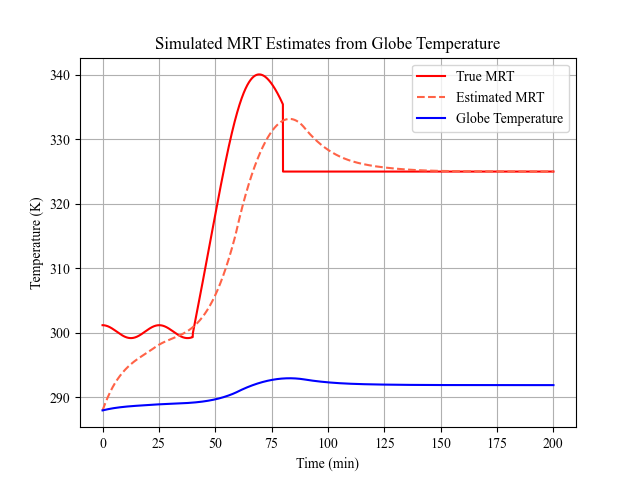
\includegraphics[width=0.75\textwidth]{First-shell-only-simulation.png}
	\caption{Illustrative simulation for MRT estimates. For this simulation we chose the following constants: wind speed $V_a = 10\unit{\meter\per\second}$, air temperature $T_a = 288 \unit{\kelvin}$, globe diameter $D = 0.15\unit{\meter}$, globe density (copper) $\rho_g = 8960 \unit{\kilogram \per\meter\cubed}$, globe emmisivity $\epsilon_{g} = 0.95$, isobaric specific heat capacity (copper) $c_{P,g} = 385 \unit{\joule \per\kilogram\per\kelvin}$ and volume (shell thickness $0.5\unit{\milli\meter}$) $V_g = 1.41 \cdot 10^{-4}\unit{\meter\cubed}$. We assumed the starting temperature of the globe was the same as the air.}
	\label{fig:first-shell-only-simulation}
\end{figure}
Figure \ref{fig:first-shell-only-simulation}  is one such simulation. Although slightly unrealistic in the continued increase of the true MRT between minute 40 and 75, it might still represent a run through a forest area, followed by a mountainous area where we steady get higher in the atmosphere and green vegetation is replaced with more reflective green rock. At the end, we could imagine the subject standing still in the same stop. This simulation illustrates the ability of this method to study both the response time in a changing and static environment. \textbf{This simulation was done numerically, and used an implicit integration scheme to account for the possible stiffness of the true MRT function.}

\subsection{Inner Temperature Simulation}
Up until now, we essentially viewed our globe temperature as the temperature the shell of our globe thermometer has. Figure \ref{fig:first-shell-only-simulation} thus simulated the shell temperature. However, a rigorous discussing of the air inside our globe thermometer is needed. After all, we measure the air temperature inside the shell $T_i$, and not the shell temperature directly. For MRT measurements in static (or very slowly varying) environments, we can assume that enough time has passed such that the air inside has the same temperature as the shell. This follows from the fact that equilibrium for the air inside (assuming a perfectly closed shell) is reached when the temperature of air is the same as that of the globe.
\\

However, when the true MRT changes, the air temperature inside the shell must first adequately change to get an accurate estimate. For this, imagine again we move from a shady to a sunny area such that our true MRT spikes. The environment will than first heat up the shell, which in turn has the heat up the air inside. This means that the simulation from figure \ref{fig:first-shell-only-simulation} represents an idealized situation, and in actuality our measured air temperature will adapt more slowly and MRT estimates will even more inaccurate. We now introduce this effect into our simulation. From now on, globe temperature $T_g$ is specifically meant to represent the shell temperature (or the actual 'globe' part of the thermometer).
\\

In the context of this bachelorproject, the globe thermometers will be constantly moving due to the nature of how people run. We can  therefore, confidently, assume that the air inside the globe is uniformly mixed at all times and the temperature evenly spread. In this case, we the change in heat over time for the air inside is given by
$$
\dot{Q}_i = A_ih_i(T_g - T_i) = n_ic_{V,i} \dot{T}_i
$$
With $A_i$ the surface of the inside of the shell and $h_i$ the convective heat transfer coefficient for the air inside. Note that we use the specific isochoric heat capacity now, because of this we must know the moles of air $n_i$ inside the globe (which we can find using the volume, density and molar mass).
\\

In order to heat up, or cool down, the air inside, there must be heat transfer between the globe and the air. Thus, we need to account for this exchange in \eqref{eq:ideal-grey}, we find that
$$\dot{Q}_g = A\left(a_g\sigma T^4_{\text{MRT}} - \epsilon_g\sigma T^4_g - h(T_g - T_a)\right) - A_ih_i(T_g - T_i) = \rho_gV_gc_{P,g} \dot{T}_g 
$$
All together we find the coupled set of equations
\begin{equation}\label{eq:realistic-simulation}
	\boxed{
	\left\{
	\begin{aligned}
		\dot{T}_i &= \frac{A_ih_i}{n_ic_{V,i}}(T_g - T_i) \\
		\dot{T}_g &= \frac{1}{\rho_gV_gc_{P,g}}\left[A\left(a_g\sigma T^4_{\text{MRT}} - \epsilon_g\sigma T^4_g - h(T_g - T_a)\right) - A_ih_i(T_g - T_i)\right]
	\end{aligned}
	\right.
	}
\end{equation}
Using these equations, we numerically simulate, figure \ref{fig:shell-and-air-simulation}, the estimated MRT with the same synthetic true MRT function as figure \ref{fig:first-shell-only-simulation}.
\begin{figure}[H]
	\centering
	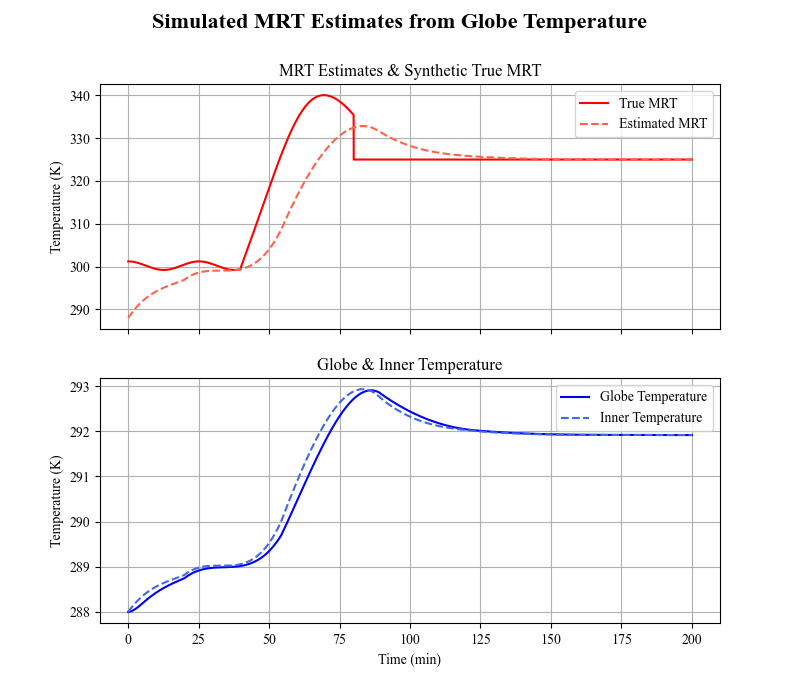
\includegraphics[width=0.75\textwidth]{Shell-and-air-simulation.png}
	\caption{Illustrative simulation for both inner air and shell. The simulated conditions were the same as figure \ref{fig:first-shell-only-simulation}. The inner temperature closely follows the globe temperature. For this simulation, we choose $h_i = 7 \unit{\joule\per\second\per\meter\squared\per\kelvin}$, which is a very conservative estimate. Higher $h_i$ yield faster adaptions of the inner air, and thus realistically the inner air follows the globe temperature even more closely. \textbf{The inner and shell temperature are labeled wrong, and should be swapped. So the dashed line is the globe temperature and the full-line is the inner temperature.}}
	\label{fig:shell-and-air-simulation}
\end{figure}
We see that the inner air temperature closely follows the globe temperature. We note that, in some sense, this is a worst case scenario simulation. Since the convective heat transfer coefficient $h_i$ has been chosen very conservatively. Depending on the running speed, this value can significantly increase, yielding faster changes in inner air temperature. Realistically, the inner air will thus even more closely follow the globe temperature. Still, we suggest to take this effect into account.

\subsection{Verification of Simulation Model Through Response Times}
In the paper "Assessment of black globe thermometers employing various sensors and alternative materials" they set out to study how various materials, sensors and diameters might influence MRT measurements. A key part of this investigation was finding the response time of each setup. We use these results to verify if they match the response times obtained through our simulation model \eqref{eq:realistic-simulation}.
\\

To achieve this, we use the response times obtained from the IR sensor. This sensor has a reported accuracy of $\pm 0.5\unit{\kelvin}$. We therefore determine the simulated 'response' by checking when our estimated MRT is within 0.5 of the true MRT. (now include the figures)


\section{Recreating the true MRT function}
From our simulations we see that direct estimation with our equation \eqref{eq:ideal-grey} isn't accurate. However, we do know that measurements are unique defined by the true MRT function. If we assume the through MRT has some form, e.g. a linear combination of basis functions, we might be able to numerically fit the coefficients of this form to best reproduce the measured data through simulation. So we estimate the coefficients of the true MRT function, we simulate our estimate using these coefficients, and we compare with the actual data. If the simulation matches, we have a good fit, otherwise we try finding better coefficients. My current though is the use either an $n$-order polynomial (so $n$ coefficients) or a fourier series.
\end{document}
